\documentclass[a4paper,12pt]{report}
\author{}
\date{}

\usepackage[shortlabels]{enumitem}
\usepackage{graphicx}
\usepackage{hyperref}
\graphicspath{ {./images/} }

\begin{document}
    \begin{titlepage}
        \begin{center}
            
            \textbf{\Large Application of AI on IT Service Management}
                
            \vspace{1.5cm}

            \begin{figure}[h]
                
\includegraphics[scale=1.0]{EPITA.jpg}
                \centering
            \end{figure}
    
            \begin{center}
                \centerline{Arun singh Sivaprakash}
                \centerline{Pramod kumar Nagaraj}
                \centerline{Van Tien NGUYEN}
                \centerline{Alexander POPPE}
            \end{center}
    
            \vfill

            \centerline{EPITA Graduate School of Computer Science}
            
                
            \begin{center}
                \centerline{Advisor}
                \centerline{ Olivier Berthet}
            \end{center}
        
            \begin{center}
                Master of Science in Artificial Intelligence Systems
            \end{center}
        
            \vfill
            \centerline{16-07-2021}
                
        \end{center}
    \end{titlepage}


    \setcounter{page}{1}
    \tableofcontents


    \chapter{Introduction}
    Here is the introduction of our Thesis

    \chapter{State of Art}
    Natural language processing (NLP) is a subfield of linguistics, computer science, and artificial intelligence concerned with the interactions between computers and human language, in particular how to program computers to process and analyze large amounts of natural language data. The goal is a computer capable of "understanding" the contents of documents, including the contextual nuances of the language within them. The technology can then accurately extract information and insights contained in the documents as well as categorize and organize the documents themselves.
    In our project, NLP is used to extract information tickets and evaluate the quality of data.

    \section{NLP pipeline}
    In general, NLP contains three main stages: text processing, feature extraction, modeling.
    
    \begin{figure}[h]
        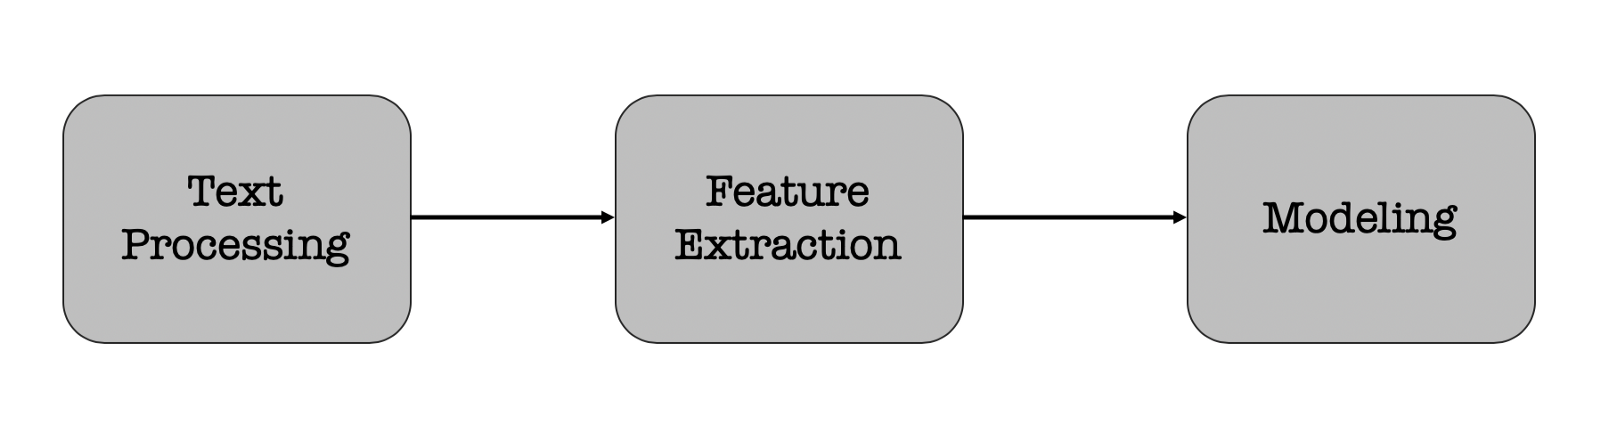
\includegraphics[scale=0.18]{nlp_pipeline.png}
        \centering
        \caption{NLP pipeline}
    \end{figure}

    \subsection{Text Processing}
    In this step, we take text raw as an input. Then we process the input into a form that is the best for next step: feature extraction.
    More specifically, raw data needs to be cleaned that means removing special characters such as HTML tags, etc. In other words, input data does not contain any info for the model to lean and are irrelevant or noisy data.
    After that, we do the data normalization which involes the case normalization, punctuation removal so that the text is in a single format for the machine to learn.
    In case normalization, we convert all capitalization to lower to bring a common case, 
    and in punctuation removal, we replace all punctuations with space.
    The next process is breaking up text documents into individual words called tokens and remove the stop words.
    Stop word removal means removing the non-important words like "a", "is", "the", "and", "an", etc. After that, we need to reduce words to its normalized form, and this process can be done by stemming or lemmatization technique.
    Stemming is a process of reducing a word to its root form, for example: "branching", "branched" and "branches" can all be reduced to "branch", 
    meanwhile lemmatization is the algorithmic process of determining the canonical
    form (lemma) of a word.
    Unlike stemming, it is not only a word reduction but depends on the
    meaning of the word in a sentence and needs to consider a language’s
    full vocabulary, for instance: "was" will be transformed into "be", "meeting" will be "meet" or "meeting" depending on the context.

    \subsection{Feature Extraction}
    Feature Extraction is a way of extracting feature vectors from the text after the text processing step so that it can be used in the machine learning model as input.
    Word Embedding is one such technique where we can represent the text using vectors. The more popular forms of word embeddings are:
    Bag-of-Words (BoW) and Term Frequency-Inverse Document Frequency (TF-IDF).
    Bow is a way of extracting features from the text for use in modeling, it treats each document as a collection or bag of word. This means a representation of text that describes the occurrence of words within a document.
    It involes two things: a vocabulary of known words in the corpus (set of documents) and a measure of the presence of known words.
    For example: we have two documents: Document1 is "Xavier likes to play football. Eric likes football too." and Document2 is "Eric prefers tennis to football", we can have the representation below:

    \begin{figure}[h]
        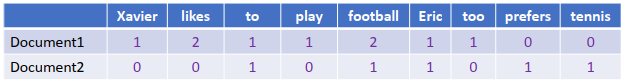
\includegraphics[scale=1.0]{bow.png}
        \centering
        \caption{Example of BoW}
    \end{figure}

    Term Frequency-Inverse Document Frequency is a ponderation method uused in information retrieval. This statistical measure gives an evaluation of how important is a word to a document, depending on the corpus considered.
    TF-IDF is calculated as: $tfidf(t,d,D) = tf(t,d) * idf(t,D)$
    Inverse document frequency:
    \begin{math}
        idf(t,D) = \log(\frac{N}{|\{d\in D:t\in d\}|})
    \end{math}
    with N the number of documents in corpus D. We continuously calculate tf-idf for the above example:

    \begin{figure}[h]
        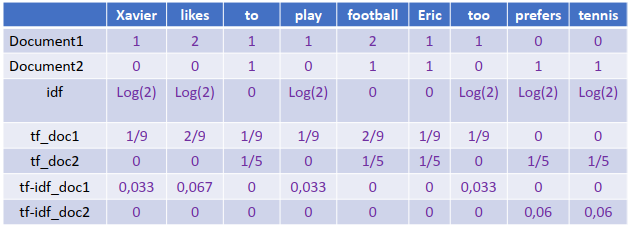
\includegraphics[scale=1.0]{tf-idf.png}
        \centering
        \caption{Example of TF-IDF calculation}
    \end{figure}

    \subsection{Modeling}
    The final stage of the NLP pipeline is modeling, which includes designing a statistical or machine learning model, 
    fitting its parameters to training data, using an optimization procedure, and then using it to make predictions about unseen data.
In our project, we use clustering machine learning algorithms. Here is an overview of this algorithm. 
Clustering is an unsupervised machine learning task. It involves automatically discovering natural grouping in data. Unlike supervised learning, clustering algorithms only interpret the input data and find natural groups or clusters in features in feature space.
A cluster is often an area of density in the feature space where examples from the domain (observations or rows of data) are closer to the cluster than other clusters. The cluster may have a center (the centroid) that is a sample or a point feature space and may have a boundary or extent.
Clustering can be helpful as a data analysis activity in order to learn more about the problem domain. It also can be useful as a type of feature engineering, where existing and new examples can be mapped and labeled as belonging to one of the identified clusters in the data.
Evaluation of identified clusters is subjective and my require a domain expert, although many clustering-specific quantitative measures do exist. Typically, clustering algorithms are compared academically on synthetic datasets with pre-defined clusters which an algorithm is expected to discover.
There are two common clustering algorithms: K-Means and Gaussian Mixture Model.
    
    \subsubsection{K-Means:} 
    This is one of the simplest and frequently used unsupervised learning algorithms, especially in data mining and statistics. Being a portioning algorithm, its goal is to form groups of data points based on the number of clusters, represented by the variable k. K needs to be predefined before the execution. K-means uses an iterative refinement method to produce its final clustering based on the number of clusters defined by the user and the dataset. Initially, k-means randomly chooses k as the mean values of k clusters, called centroids, and find the nearest data points of the chosen centroids to form k clusters. Then, it iteratively recalculates the new centroids for each cluster until the algorithm converges to one optimum value. K-means clustering would be suited with the numerical data with a low dimensionality because numerical data is used to compute the mean value. The type of data best suited for K-means clustering would be numerical data with a relatively lower number of dimensions.
    \newline
    Problem description: A set of observations $(x_1, x_2, …, x_n)$ where each observation is a $d$-dimensional real vector, this algorithm aims to partition the n observations into $k(<=n)$ sets $S = \{S_1, S_2, …, S_k\}$ so as to minimize the within cluster sum of squares.
    \newline
    Algorithm: initial randomly set of k means $(m_1, m_2, …, m_k$, the algorithm proceeds by altering between two steps.
    The first step is assignment step: assign each observation to the cluster with the nearest mean that with the least squared Euclidean distance:
    $S_i = \arg\min\limits_k||x_i - m_k||^2$. 
    The second step is update step which recalculates the means (centroids) for observation assigned to each cluster:
    $m_k = \frac{\Sigma_{i:k_i=k}x_i}{|i:k_i=k|}$.
    The algorithm has converged when the assignments no longer change.
    \newline
    K-means has some advantages which are simple clustering algorithm so that it can be implemeneted easily. It also faster computationally than other clustering algorithms because K-means has only a few comupations.
    Additionally, this algorithm can scale up to large dataset and easily adapt to new data samples.
    Besides, there are some disavantages: K-means has difficulty with clustering data set of varying sizes and density. Its result can also vary depending on inital values and the number is clusters has to be specified manually.    

    \subsubsection{Gaussian Mixture Model (GMM): }
    Probabilistic models and use the soft clustering approach for distributing the points in different clusters, it assumes that there are a certain number of Gaussian distributions and each of these distributions represent a cluster. therefore, a GMM tends to group the data points belonging to a single distribution together.
    \newline
    Gaussian distribution (or Normal distribution): is a type of continuous probability distribution for a real-valued random variable. The general form of its probability density function:
    $f(x) = \frac{1}{\sigma \sqrt{2\pi}}e^{-\frac{(x-\mu)^2}{2\sigma^2}}$, with parameters: $\mu$ is mean of the distribution and $\sigma$ is standard deviation.
    \newline
    To implement GMM, we use Expectation-Maximization algorithm (EM). EM is a statistical algorithm for finding the right model parameters.
    It typically used for handling missing values or in other words latent variables. This algorithm has two steps: E-step, the available data is used to estimate the values of the missing variables
    and M-step, based on the estimated values generated in the e-step, the complete data is used to update the parameters.
    \newline
    EM in GMM: We need to assign k number of clusters. This means that there are k Gaussian distributions, with the mean and covariance values to be $\mu_1, \mu_2, ..., \mu_k$
    and $\sigma_1, sigma_2, ..., sigma_k$. Additionally, there is another parameter for the distribution that defines the number of points for the distribution. Or in other words, the density of the distribution is represented with $\Pi$


    \chapter{System's Artchitecture}

    
    \chapter{Methodology}


    
    \chapter{Results}


    
    \chapter{Conclusion}

    
    \chapter{References}


    \begin{thebibliography}{9}
        \bibitem{wikipedia website}
        \href{https://en.wikipedia.org/wiki/Natural_language_processing}{Wikipeida: Natural language processing}

        
        \bibitem{website}
        \href{https://www.gyansetu.in/what-is-natural-language-processing/}{Article: iClass Gyansetu}
    \end{thebibliography}

\end{document}